% updated April 2002 by Antje Endemann
% Based on CVPR 07 and LNCS, with modifications by DAF, AZ and elle, 2008 and AA, 2010, and CC, 2011; TT, 2014; AAS, 2016; AAS, 2020

\documentclass[runningheads]{llncs}
\usepackage{graphicx}
\usepackage{comment}
\usepackage{amsmath,amssymb} % define this before the line numbering.
\usepackage{color}

\usepackage[binary-units]{siunitx}

% TODO setup camera ready document
\newif\ifcamera
%\cameratrue
\camerafalse


\ifcamera
% Do nothing
\else
\usepackage{ruler}
\usepackage[width=122mm,left=12mm,paperwidth=146mm,height=193mm,top=12mm,paperheight=217mm]{geometry}
\fi

\title{Error-Free Semantic Segmentation Inference of Images Larger than GPU Memory}

\pagestyle{headings}
\mainmatter
\def\ECCVSubNumber{5548}  % Insert your submission number here

\ifcamera
% CAMERA READY SUBMISSION
%******************
\titlerunning{Error-Free Out-of-Core FCNN Inference}
% If the paper title is too long for the running head, you can set
% an abbreviated paper title here

%\author{First Author\inst{1}\orcidID{0000-1111-2222-3333} \and
%Second Author\inst{2,3}\orcidID{1111-2222-3333-4444} \and
%Third Author\inst{3}\orcidID{2222--3333-4444-5555}}

\author{Michael Majurski\inst{1} \and Peter Bajcsy\inst{1}}

\authorrunning{M. Majurski and P. Bajcsy}
% First names are abbreviated in the running head.
% If there are more than two authors, 'et al.' is used.
%
\institute{National Institute of Standards and Technology\\
	Information Technology Lab\\
	Gaithersburg, MD 20899, USA\\
	\email{\{michael.majurski,peter.bajcsy\}@nist.gov}}

%******************
\else
% INITIAL SUBMISSION 
%******************
\titlerunning{ECCV-20 submission ID \ECCVSubNumber} 
\authorrunning{ECCV-20 submission ID \ECCVSubNumber} 
\author{Anonymous ECCV submission}
\institute{Paper ID \ECCVSubNumber}
%******************
\fi



\begin{document}


\maketitle
 
%%%%%%%%% ABSTRACT
\begin{abstract}

We address the problem of performing error-free out-of-core semantic segmentation inference of arbitrarily large images using fully convolutional neural networks (FCNN). FCNN models have the property that once a model is trained it can be applied on arbitrarily sized images, though it is still constrained by the available memory (RAM) of the GPU executing the inference. This work is motivated by overcoming the GPU memory size constraint via a tile-based inferencing methodology which does not numerically impact the final result. This enables inference of whole slide microscopy images generated by a slide scanner, for example.

We documented the mathematical formulas for determining the tile size and stride of tiles created from an input image too large to inference on a GPU. 
The formulas are validated on U-Net and FC-DenseNet architectures.
The numerical accuracy is evaluated on a GPU with 24 GB of RAM that can inference tiles as large as $\num{3584} \times \num{3584}$ pixels while the whole input images are $\num{20000} \times \num{20000}$ pixels. 

This method decomposes the full inference image into small, overlapping tiles; each of which fit into GPU memory for the forward (inference) pass of the network. 
This tiling scheme produces a segmentation result as if the whole image had been inferenced in a single pass. 
The primary contribution of this work lies in demonstrating that one can achieve error-free inference using a tile-based (out-of-core) approach if the tiling parameters are chosen according to the mathematical analysis of the FCNN model. 
In addition, we document the errors due to tiling configurations which do not satisfy the constraints, and explore using architecture effective receptive fields to estimate the tiling parameters. 

\end{abstract}

%%%%%%%%% BODY TEXT
\section{Introduction}

The task of semantic segmentation, assigning a label to each image pixel, is often performed using deep learning based convolutional neural networks (CNNs) \cite{Badrinarayanan2015a,Ronneberger2015a}, for instance, by using a special type of CNN which only uses convolutional layers.
These so-called "fully convolutional neural networks" (FCNN) have a very useful property which allows the alteration the input image size. 
Both U-Net \cite{Ronneberger2015a} and the original FCN network \cite{Long2015} are examples of FCNN type CNNs. 
FCNNs enable training the network on images much smaller than those of interest at inference time. 
For example, one can train a U-Net model on $512 \times 512$ pixel tiles and then perform GPU-based inference on arbitrary pixel sized images as long a the RAM of a GPU can accommodate the U-Net model coefficients, the network activations, application code, and an image tile to be inferred. This decoupling of training and inference image sizes means the semantic segmentation models can be applied to images much larger than the memory available on current GPUs. 

The ability of FCNN networks to inference arbitrarily large images differs from other types of CNNs where the training and inference image sizes must be identical. Usually this static image size requirement is not a problem since the input images can be resized to fit the network. For example, if one trained a CNN on ImageNet \cite{Russakovsky2015} to classify pictures into two classes: \{Cat, Dog\}, the content of the image does not change drastically if the cat photo is resized to $224 \times 224$ pixels before inference.

%In another example, performing semantic segmentation of the scene acquired by a self driving car's front camera, one can infer which surfaces are drivable at the native camera resolution of 720p ($1280 \times 720$ pixels $\sim \SI{1}{\mega pixel}$). Alternatively, one can inference images after down-samplings if compute time must be decreased in such a time-critical application. 

In contrast, there are applications where resizing (re-scaling or down-sampling) the image is not acceptable due to loss of information. For example, in digital pathology, one cannot take a whole slide microscopy image generated by a slide scanner (upwards of $\num{10}$ Gigapixels) and fit it into GPU memory; nor can one reasonably resize the image as too much image detail would be lost. 

Our work is motivated by the need to design a methodology for arbitrarily large image inference on GPU memory constrained hardware in those applications where the loss of information due to image resizing is not acceptable. The original U-Net paper \cite{Ronneberger2015a} briefly hinted at the feasibility of an inference scheme similar to the one we present in this paper but did not fully document and explain the inference scheme. 
The novelty of our work lies in presenting a methodology for error-free inference over images that are larger than available GPU memory for processed data. This work leverages FastImage \cite{Bardakoff2019}, a high-performance accessor library for processing gigapixel images in a tile-based manner.

\section{Related Work}
\label{related-work}

It has been known since the initial introduction of fully convolutional neural networks that they can be applied via shift-and-stitch methods as if the FCNN were a single filter \cite{Long2015,Sherrah2016}.
The original U-Net paper by Ronneberger et al. \cite{Ronneberger2015a} also hints at inference of arbitrary sized images in its Figure 2. However, none of the past papers mentioning shift-and-stitch discuss the methodology for performing out-of-core arbitrary sized image inference.

There are two common approaches for applying CNN models to large images: sliding window (overlapping tiles) and patch-based inference. Sliding window (i.e. overlapping tiles) has been used for object detection \cite{Sermanet2013,VanEtten2019} as well as for semantic segmentation \cite{Lin2019,Volpi2017a} inference. Patch-based inference also supports arbitrarily large images, but it is very inefficient \cite{Volpi2017a,Maggiori2016}.

Huang et al. directly examine the problem of operating on images which cannot be inferenced in a single forward pass. However, the authors focus on different methods for reducing the error in labeling that arises from different overlapping tile-based processing schemes \cite{Huang2019a}. They examine label averaging and the impacts of different tile sizes on the resulting output error and conclude that using as large a tile as possible will minimize the error \cite{Huang2019a}. Huang et al. also examine the effects of zero-padding, documenting how much error it introduces \cite{Huang2019a}. At no point do they produce error-free tile-based inference. Iglovikov et al. also remark upon error in the logits near the edge of tiles during inference and suggest overlapping predictions or cropping the output to reduce that error \cite{Iglovikov2017}. 

Our ability to perform error-free tile-based inference relies on the limited receptive field of convolutional layers as explored by Luo et al. \cite{Luo2016}. Luo et al. \cite{Luo2016} discuss the receptive fields of convolutional architectures, highlighting that for a given output pixel, there is limited context/information from the input that can influence that output. Input data outside the receptive field cannot influence that output pixel \cite{Luo2016}. The receptive field of a model is highly dependent upon architecture and layer connectivity. We us the theoretical underpinning of receptive fields to identify a sufficient size of an image tile for error-free inference.  

To the best of our knowledge, no published method fully explores a methodology for error-free tile-based (out-of-core) inference of arbitrarily large images. While tile-based processing schemes have been outlined, the past publications do not provide a framework for achieving error-free tile-based inference results.


\section{Methods}
\label{methods}

To explain out-of-core image inference we use U-Net \cite{Ronneberger2015a} as the case study FCNN. Nonetheless, the presented methodology applies to any FCNN network, just the specific numerical values will be different. 

\subsection{U-Net Configuration}

Before delving into the out-of-core inference methodology details, we clarify two modifications of U-Net. 

\begin{enumerate}
	\item Normalization: Batch normalization \cite{ioffe2015batch} was added after the activation function of each convolutional layer as it is current good practice in the CNN modeling community. 
	\item Convolution Type: Convolutional type was changed to \texttt{SAME} from \texttt{VALID} as used in the original paper \cite{Ronneberger2015a}.
\end{enumerate}

The original U-Net paper uses \texttt{VALID} type convolutions which shrink the spatial size of the feature maps by 2 pixels for each layer \cite{Dumoulin2018}\footnote{For an excellent review of convolutional arithmetic, including transposed convolutions (i.e., up-conv), see "A guide to convolutional arithmetic for deep learning by Dumoulin and Visin" \cite{Dumoulin2018}.}. 
%Figure 2.1 from Dumoulin and Visin "A guide to convolutional arithmetic for deep learning" \cite{Dumoulin2018} shows an illustration showing why \texttt{VALID} causes the feature maps to shrink. The effect of \texttt{VALID} convolutions can also be seen in the first layer of the original U-Net where the input image size of $572 \times 572$ pixels shrinks to $570 \times 570$ \cite{Ronneberger2015a}. 
Switching to \texttt{SAME} type convolutions requires that within each convolutional layer zero padding is applied to each feature map to ensure the output has the same spatial size as the input. 
%Figure 2.3 from Dumoulin and Visin \cite{Dumoulin2018} shows an illustration where a input $5 \times 5$ remains $5 \times 5$ after the convolution is applied. 
While \texttt{VALID} type convolutions avoid the negative effects of the zero padding within \texttt{SAME} type convolutions, which can affect the results as outlined by Huang et al. \cite{Huang2019a}, users prefer input and output images of the same size. Additionally, our tiling scheme overcomes all negative effects that zero padding can introduce, justifying the choice of \texttt{SAME} type convolutions. 

The change to \texttt{SAME} type convolutions introduces an additional constraint on U-Net that needs to be mentioned. Given the skip connections between the encoder and decoder elements for matching feature maps, we need to ensure that the tensors being concatenated together are the same size. The feature map at the bottleneck of U-Net is spatially $16 \times$ smaller than the input image. 
As we go deeper into a network we trade spatial resolution for feature depth. Given a $512 \times 512$ pixel input image, the bottleneck shape will be $N \times 1024 \times 32 \times 32$ (assuming \texttt{NCHW}\footnote{NCHW Tensor dimension ordering: N (batch size), Channels, Height, Width} dimension ordering with unknown batch size). Thus the input image height divided by the bottleneck feature map height is $\frac{512}{32} = 16$. However, if the input image is $500 \times 500$ pixels, the bottleneck would be (in theory) $N \times 1024 \times 31.25 \times 31.25$. When there are not enough input pixels in a feature map to perform the $2 \times 2$ max pooling, the output feature map size is the floor of the input size divided by $2$. 
Thus, for an input image of $500 \times 500$ pixels the feature map heights after each max pooling layer in the encoder are: [$500, 250, 125, 62, 31$]. Now following the up-conv (fractionally strided/transposed convolution \cite{Dumoulin2018}) layers through the decoder, each of which doubles the spatial resolution, we end up with the following feature map heights: [$31, 62, 124, 248, 496$]. This results in a different feature map spatial size at the third level; encoder 125, decoder 124. If the input image size is a multiple of $16$ this mismatch cannot happen. 

To ensure the input image is always a multiple of 16, we pad the end of each spatial dimension via reflection to meet the size requirement. So a $500 \times 500$ pixel image will be padded on the right and bottom with 12 pixels to bring its size to $512 \times 512$ pixels. Conversely, a $512 \times 512$ pixel image will be inferenced unmodified. Reflection padding is used to ensure that the summary statistics of the whole image are not unduly skewed since z-score normalization is used during inference. 
For the purpose of brevity, we will use 'up-conv' (as the U-Net paper does) to refer to fractionally strided convolutions with a stride of $\frac{1}{2}$ which double the feature map spatial resolution \cite{Dumoulin2018}.

\subsection{Conceptual Framework}

Given an FCNN model architecture and a GPU with enough memory to inference at least a $512 \times 512$ pixel image, we can construct a scheme for inferencing arbitrarily sized images. There are two important concepts required for this tile-based (out-of-core) processing scheme. 
\begin{enumerate}
	\item Zone of Responsibility (ZoR): a rectangular region (partition, zone, or area) of the output image currently being computed.
	\item Radius: minimum horizontal and vertical border size around the ZoR indicating the local context that the FCNN requires to accurately compute all pixels within the ZoR.
\end{enumerate}

Each dimension of a square tile is then defined as $TileSize = ZoR + 2 \times Radius$. 
Figure \ref{fig:zor} shows an example where a $832 \times 832$ pixel zone of responsibility is shown as a square with a $96$ pixel radius surrounding it. 
Since the pixels within the ZoR and the radius need to be passed through the network to compute the output, one tile of GPU input is $832 + 2 \times 96 = 1024$ pixels per spatial dimension.

\begin{figure}[h!]
	\centering
		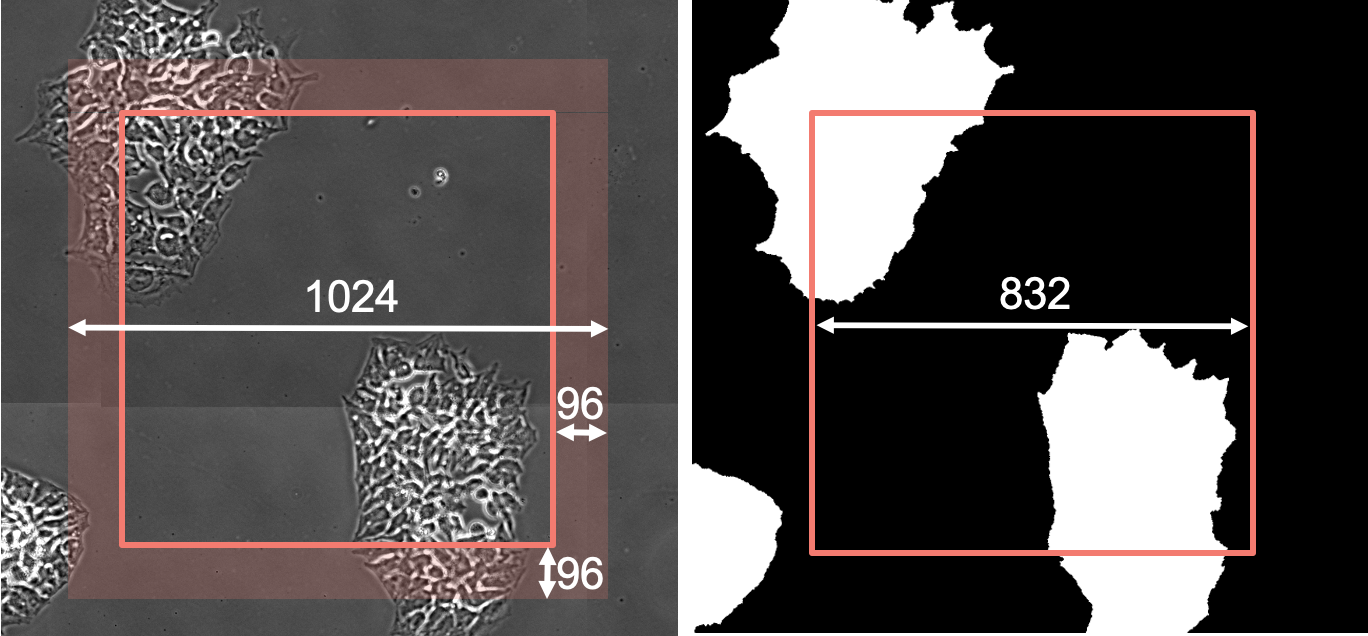
\includegraphics[width=\linewidth]{figs/zor.png}
	\caption{Left: ZoR ($832 \times 832$ pixel square) with a $96$ pixel surrounding radius (shaded area) for tile-based inference of stem cell colonies. Right: segmentation output showing the ZoR contribution.}
	\label{fig:zor}
\end{figure}

Inferencing arbitrarily large input images requires that we inference only a small enough tile to fit in GPU memory for any single forward pass and then operate tile-by-tile. To form a tile, the whole image being inferenced is broken down into non-overlapping zones of responsibility. For each ZoR, the local context defined by the radius (where that context is available) is included and passed through the network. The ZoR within the inferenced tile result (without the radius) is copied to the output image being constructed in CPU memory. The radius provides the network with all the information it needs to make correct, deterministic predictions for the entirety of the zone of responsibility. 
%Hence the name, since each ZoR is responsible for a specific zone of the output. 
Therefore, while the full image was broken into tiles for inference, each pixel had all of the local context required to be predicted as if the whole image were passed through the network as one block of memory. 

This tile-based inferencing can be thought of as a series of forward passes, each computing a subregion (ZoR) of the feature maps that would be created while inferencing the whole image in one pass. 
In summary, each tile's feature maps are created (inferenced), its ZoR output extracted, and then the GPU memory is recycled for the next tile. By building each ZoR in a separate forward pass we can construct the network output within a fixed GPU memory footprint for arbitrarily large images. 


\subsection{Determining The Radius}

%\begin{figure*}[h!]
%	\centering
%		\includegraphics[width=\linewidth]{figs/unet-levels.png}
%	\caption{U-Net model architecture showing the different convolutional layers (blue arrows) and their respective levels. Each blue box is a multi-channel feature map with the channel count denoted on top of the box and the spatial dimension at the lower left edge. White boxes represent copied and concatenated feature maps. Each convolutional layer is numbered sequentially along the longest path through the network from input image to output segmentation result.}
%	\label{fig:unet-levels}
%\end{figure*}

Let U-Net be described by an ordered sequence of convolutional layers $c={0, ..., N-1}$ with each layer being associated with a level $l_{c}$ and a square kernel $k_{c} \times k_{c}$. 
A convolutional layer (1) convolves a kernel and its input feature maps to create a set of output feature maps, (2) applies an element-wise a non-linearity (ReLu \cite{lecun2015deep}), and (3) performs batch normalization \cite{ioffe2015batch} on its output feature maps.
For the network, $N$ defines the number of convolutional layers along the longest path from input to output. 
%The index of $c$ for each convolutional layer is written on each blue arrow in Figure \ref{fig:unet-levels}.

Let us define the level $l_{c}$ of an encoder-decoder network architecture as the number of max-pool\footnote{Convolutions with a stride of 2 can also be used to halve the spatial size of the feature maps.} layers minus the number of up-conv layers between the input image and the current convolutional layer $c$ along the longest path through the network. Levels start at 0; each max pool encountered along the longest path increases the level by 1 and each up-conv reduces the level by 1. 


\subsubsection{General Radius Calculation}
The minimum required radius can be calculated according to the Equation \ref{eq:radius} for a general FCNN architecture. 

\begin{equation}
Radius = \sum_{c=0}^{N-1} 2^{l_c} \lfloor \frac{k_c}{2} \rfloor
\label{eq:radius}
\end{equation}

The radius is a sum over every convolutional layer index $c$ from $0$ to $N-1$ encountered along the longest path from the input image to the output.
Equation \ref{eq:radius} has two terms. The $2^{l_c}$ term is the number of pixels at the input image resolution that correspond to a single pixel within a feature map at level $l_c$. Therefore, if a $3 \times 3$ convolution is applied at level $l_c=4$ then $2^4 = 16$ pixels of context are needed at the input image resolution. This $2^{l_c}$ term is multiplied by the second term $\lfloor \frac{k_c}{2} \rfloor$ which determines, for a given $c$, how many pixels of local context are required at that feature map resolution to perform the convolution.

\subsubsection{Radius Calculation for U-Net}

%Let us assume that the U-Net architecture satisfies the following design constraints: $k_c = k = const$ and each level has the same number of convolutional layers on both decoder and encoder sides $n_l = n = const$. These constraints are satisfied for the published U-Net where $k = 3$ and $n_l = 2$.

%In this case, the minimum required radius can be calculated according to the Equation \ref{eq:radius2}, 
%\begin{equation}
%Radius = \lfloor \frac{k}{2} \rfloor \times n \times (3 \times 2^{M} - 2)
%\label{eq:radius2}
%\end{equation}
%where $M$ is the maximum level value $l_c$ over all values of $c$ (i.e., $M=max_{\forall c} (l_c)$). The radius is linearly proportional to the kernel size $k$ and to the number of convolutional layers per level $n$ and exponentially proportional to the maximum level $M$. The derivation of Equation \ref{eq:radius2} from Equation \ref{eq:radius} is provided in Appendix A.

The published U-Net (Figure 1 from \cite{Ronneberger2015a}) has one level per horizontal stripe of layers. The input image enters on level $l_{c=0} = l_{c=1} = 0$. The first max-pool layer halves the spatial resolution of the network, changing the level. Convolution layers $c = \{2, 3\}$ after that first max-pool layer up to the next max-pool layer belong to level $l_{c=2}=l_{c=3} = 1$. This continues through level 4, where the bottleneck of the U-Net model occurs. In U-Net's Figure 1 \cite{Ronneberger2015a}, the bottleneck is the feature map at the bottom which occurs right before the first up-conv layer. After the bottleneck, the level number decreases with each subsequent up-conv layer, until level $l_{N-1} = 0$ right before the output image is generated. 

The radius computation in Equation \ref{eq:radius} can be simplified for U-Net as shown in Appendix A. Appendix B shows a numerical example for compute a radius using Equation \ref{eq:radius}.

Following Equation \ref{eq:radius} for U-Net results in a minimum required radius of 92 pixels in order to provide the network with all of the local context it needs to predict the outputs correctly. This radius needs to be provided both before and after each spatial dimension and hence the input image to the network will need to be $2 \times 92 = 184$ pixels larger. This value is exactly the number of pixels the original U-Net paper has the output being shrunk by to avoid using \texttt{SAME} convolutions; a 572 pixel input shrunk by 184 results in the 388 pixel output \cite{Ronneberger2015a}. 
However, this runs afoul of our additional restriction on the U-Net input size, which requires images to be a multiple of 16. So rounding up to the nearest multiple of 16 results in a radius of 96 pixels. Since  one cannot just adjust the ZoR size to ensure $(ZoR + Radius) \% 16 = 0$ due to convolutional arithmetic, we must explore constraints on image partitioning. 

\subsection{Constraints on Image Partitioning}

Our tile-based processing methodology operates on the principle of constructing the intermediate feature map representations within U-Net in a tile-based fashion, such that they are numerically identical to the whole image being passed through the network in a single pass. Restated another way, the goal is to construct an input image partitioning scheme such that the zone of responsibility is building a spatial subregion of the feature maps that would exist if the whole image were passed through the network in a single pass. 

\subsubsection{Stride Selection}
To properly construct this feature map subregion one cannot stride across the input image in a different manner than would be used to inference the whole image. The smallest feature map in U-Net is spatially $16 \times$ smaller than the input image. Therefore, 16 pixels is the smallest offset one can have between two tile-based inference passes while having both collaboratively build subregions of a single feature map representation. Figure \ref{fig:offset} shows a simplified 1D example with a kernel of size 3 performing addition. When two applications of the same kernel are offset by less than the size of the kernel they can produce different results. 
%The output in the first row is \{$6, 15$\} whereas the output in the second row is \{$9, 18$\}. 
For U-Net, each $16 \times 16$ pixel block in the input image becomes a single pixel in the lowest spatial resolution feature map. A stride other than a multiple of 16 would result in subtly different feature maps because each feature map pixel was constructed from a different set of $16 \times 16$ input pixels. 

\begin{figure}[h!]
	\centering
		\includegraphics[width=\linewidth]{figs/partitioning.png}
	\caption{A (left): Simplified 1D example of an addition kernel of size 3 being applied at an offset less than the kernel size, producing different results (compare top and bottom sums of 1, 2, and 3 or 2, 3, and 4).
	B (right): Simplified 1D example of reflection padding (reflected through dotted line) causing a different stride pattern across a set of pixels. The altered stride prevents the tile-based processing from collaboratively building subregions of a single feature map.}
	\label{fig:offset}
\end{figure}

This requirement means that we always need to start our tiling of the full image at the top left corner and stride across in a multiple of 16. However, this does not directly answer the question as to why we cannot have a non-multiple of 16 radius value. 

\subsubsection{Border Padding}
The limitation on the radius comes from the fact that if we have arbitrary radius values, we will need to use different padding schemes between the full image inference and the tile-based inference to handle the image edge effects. Figure \ref{fig:offset} shows for a 1D case how reflection padding can (1) alter the stride across the full image which needs to be maintained as a multiple of 16 to collaboratively build subregions of a single feature map and (2) change the reflection padding required to have an input image whose spatial dimensions are a multiple of 16. Reflection padding is preferred since it preserves image statistics locally.

\subsubsection{ZoR and Radius Constraints}

Both problems, (1) collaboratively building feature maps and (2) different full image edge reflection padding requirements disappear if both the zone of responsibility and the radius are multiples of 16. Thus, we constrain the final values of ZoR and radius to be the closest higher multiple of the ratio $F$ between the image size $I$ and minimum feature map size (Equation \ref{eq:constraints}) where $F=16$ for the published U-Net, 
\begin{equation}
\begin{aligned}
F = \frac{ \min\{H_{I}, W_{I} \} }{ \min_{\forall l_{c}} \{ H_{l_{c}}, W_{l_{c}} \} } \\
Radius^{*} = F \lceil \frac{Radius}{F} \rceil \\
ZoR = F \lceil \frac{ZoR}{F} \rceil 
\end{aligned}
\label{eq:constraints}
\end{equation}
where $H_{I}$ and $W_{I}$ are the input image height and width dimensions, $Radius^{*}$ is the adjusted radius value to accommodate stride constraints, and $H_{l_{c}}$ and $W_{l_{c}}$ are the feature map height and width dimensions. 

\section{Experimental Results}
\label{experimental-results}

\subsection{Dataset}
\label{dataset}

We used a publicly accessible dataset acquired in phase contrast imaging modality and published in \cite{Bhadriraju2016}. 
The dataset consists of three collections, each with around 161 time-lapse images at roughly $\num{20000} \times \num{20000}$  pixels per stitched image frame with 2 bytes per pixels. 


\subsection{Error-Free Tile-Based Inference Scheme}

Whether inferencing the whole image in a single forward pass or using tile-based processing, the input image size needs to be a multiple of 16 as previously discussed. Reflection padding is applied to the input image to enforce this size constraint before the image is decomposed into tiles. 
%When a whole image is inferenced in a single forward pass the image size needs to be a multiple of 16. To achieve this reflection padding is used when required on the bottom and right of the image to extend its size. The same size requirement exists when performing tile-based processing. 

Let us assume that we know how big an image we can fit into GPU memory, for example $1024 \times 1024$ pixels. Additionally, given that we are using U-Net we know that the required radius is 96 pixels. Then our zone of responsibility is $ZoR = 1024 - 2 \times Radius = 832$ pixels per spatial dimension. 
%Refer back to Figure \ref{fig:zor} for a visual. 
Despite inferencing $1024 \times 1024$ pixel tiles on the GPU per forward pass, the stride across the input image is 832 pixels because we need non-overlapping ZoR. 
%Figure \ref{fig:all-zor} shows a full image with 6 non-overlapping ZoR in alternating colors (red and blue) with each radius as a shaded region surrounding each ZoR. 
The edges of the full image do not require radius context to ensure identical results when compared with a single inference pass. Intuitively, the true context is unknown since it's outside the existing image.

%\begin{figure}[h!]
%	\centering
%		\includegraphics[width=\linewidth]{figs/all_zor.png}
%	\caption{Non-overlapping ZoR with radius shown in the interior of a large image being inferenced. Each ZoR (denoted with a line) has a shaded radius region outside the square. }
%	\label{fig:all-zor}
%\end{figure}

%Image tiling starts at $[x_{st}, y_{st}, x_{end}, y_{end}] = [0, 0, 832, 832]$ and proceeds across the image with stride 832. 
In the last row and column of tiles, there might not be enough pixels to fill out a full $1024 \times 1024$ tile. However, because U-Net can alter its spatial size on demand, as long as the tile is a multiple of 16 a narrower (last column) or shorter (last row) tile can be used. 


\subsection{Errors due to Small Radius}

To experimentally confirm that our out-of-core image inference methodology does not impact the inference results we determined the largest image we could inference on our GPU, performed the forward pass, and saved the resulting softmax output values as ground truth data. We then inference the same image using our tiling scheme with varying radius values. We show that there are numerical differences (greater than floating point error) when using radius values less 96. 

We trained our U-Net model to perform binary (foreground/background) segmentation of the phase contrast microscopy images. The largest image we could inference on our GPU with $\SI{24}{\giga\byte}$ of memory is $3584 \times 3584$ pixels. We created 20 reference inference results by cropping out $K = 20$ random $3584 \times 3584$ subregions of the dataset. 

We performed tile-based out-of-core inference for each of the 20 reference images using a tile size of 512 pixels, meeting the multiple of 16 constraint. Radius values from 0 to 96 pixels were evaluated in 16 pixel increments. 

The tiling codebase seamlessly constructs the softmax output in CPU memory as if the whole image had been inferenced as a single forward pass. So our evaluation methodology consists of looking for differences in the output softmax produced by the reference forward pass ($R$) as well as the tile-based forward pass ($T$). We used the following two metrics for evaluation: Root Mean Squared Error (RMSE, Equation \ref{eq:rmse}) of the softmax and Misclassification Error (ME, Equation \ref{eq:me}) of the resulting binary segmentation masks. %ME is the number of misclassified pixels, which provides a very intuitive understanding of the error since it directly measures how many output pixels were incorrect. 
We also include Normalized Misclassification Error (NME, Equation \ref{eq:nme}), the ME normalized by the number of pixels; and Relative Runtime, where compute time to perform inference is shown relative by the runtime without the tiling scheme. This runtime highlights that there is a tradeoff to be made between the error introduced due to the out-of-core GPU inference and the compute overhead required to do so. The NME metric can be multiplied by $100$ to compute the percent of pixels with errors due to the tiling scheme.
All metrics are averaged across the $K = 20$ reference images.

\begin{equation}
RMSE = \frac{1}{K} \sum_{i=1}^{K} \sqrt{ \frac{\sum_{i = 1}^{m} \sum_{j = 1}^{n} (R_{ij} - T_{ij})^2}{mn}}
\label{eq:rmse}
\end{equation}

\begin{equation}
ME = \frac{1}{K} \sum_{i=1}^{K} \left( \sum_{i = 1}^{m} \sum_{j = 1}^{n} [ R_{ij} \neq T_{ij} ] \right) 
% https://en.wikipedia.org/wiki/Iverson_bracket
\label{eq:me}
\end{equation}

\begin{equation}
NME = \frac{1}{K} \sum_{i=1}^{K} \left( \frac{\sum_{i = 1}^{m} \sum_{j = 1}^{n} [ R_{ij} \neq T_{ij} ]}{nm} \right) 
% https://en.wikipedia.org/wiki/Iverson_bracket
\label{eq:nme}
\end{equation}

The total inference error is a composite of model error (what is directly minimized by gradient descent during training) and tiling error. We demonstrate a zero error contribution from tiling in the case of trained and untrained U-Net models (or minimum and maximum inference errors due to a model).
  
For the trained model, the error metrics are shown in Table \ref{tab:tile_size_512} with 512 pixel tiles. Once the required 96 pixel radius is met the RMSE falls into the range of floating point error and ME goes to zero. Beyond the minimum required radius, all error metrics remain equivalent to the minimum radius. The first row shows the data for the whole image being inferenced without the tiling scheme. 
The ME metric is especially informative, because when it is zero, the output segmentation results are identical regardless of whether the whole image was inferenced in a single pass or it was decomposed into tiles. Table \ref{tab:tile_size_512} highlights the engineering tradeoff that must be made, obtaining zero inference error requires $2.69 \times$ the wall clock runtime. The normalized error (NME) with naive tailing is $\num{6.1e-4}$ or $\num{0.06} \%$. Depending on your application, this level of error might be acceptable despite the potential for edge effects between the non-overlapping tiles. One consideration, larger tile sizes are more compute efficient because the ratio of the ZoR area to the tile area increases. 

\begin{table}[h!]
	\centering
\caption{Error Metrics for Tile Size 512}
\label{tab:tile_size_512}
\begin{tabular}{r|r|r|r|r|r|r}
	TileSize & ZoR & Radius & RMSE    & ME & NME & RelativeRuntime \\ 
	\hline
3584 & n/a & n/a & 0.0 & 0.0 & 0.0 & 1.0 \\
512 & 512 & 0 & $\num{1.11e-02}$ & 7773.4 & $\num{6.1e-04}$ & 1.08 \\
512 & 480 & 16 & $\num{6.35e-03}$ & 5455.4 & $\num{4.2e-04}$ & 1.31 \\
512 & 448 & 32 & $\num{3.29e-03}$ & 2372.2 & $\num{1.8e-04}$ & 1.36 \\
512 & 416 & 48 & $\num{1.95e-03}$ & 1193.7 & $\num{9.3e-05}$ & 1.61 \\
512 & 384 & 64 & $\num{7.79e-04}$ & 434.1 & $\num{3.4e-05}$ & 1.85 \\
512 & 352 & 80 & $\num{1.50e-04}$ & 71.6 & $\num{5.6e-06}$ & 2.21 \\
512 & 320 & 96 & $\num{4.17e-10}$ & 0.0 & 0.0 & 2.58 \\
\end{tabular}
\end{table}

For the untrained model, results are shown in Table \ref{tab:tile_size_1024} with 1024 pixel tiles. The results were generated using an untrained 4 class U-Net model, whose weights were left randomly initialized. Additionally, the image data for that result was normally distributed random noise with $\mu = 0, \sigma = 1$. The error coming from tile-based processing is zero once the required radius is met.

\begin{table}[h!]
	\centering
\caption{UnTrained U-Net Error Metrics for Tile Size 1024}
\label{tab:tile_size_1024}
\begin{tabular}{r|r|r|r|r|r|r}
	TileSize & ZoR & Radius & RMSE    & ME & NME & RelativeRuntime \\ 
	\hline
3584 & n/a & n/a & 0.0 & 0.0 & 0.0 & 1.0 \\
1024 & 1024 & 0 & $\num{2.36e-04}$ & 21856.9 & $\num{1.7e-03}$ & 1.08 \\
1024 & 992 & 16 & $\num{1.05e-06}$ & 234.8 & $\num{1.8e-05}$ & 1.23 \\
1024 & 960 & 32 & $\num{1.92e-07}$ & 49.7 & $\num{3.9e-06}$ & 1.30 \\
1024 & 928 & 48 & $\num{5.47e-08}$ & 13.2 & $\num{1.0e-06}$ & 1.35 \\
1024 & 896 & 64 & $\num{1.44e-08}$ & 2.8 & $\num{2.1e-07}$ & 1.31 \\
1024 & 864 & 80 & $\num{5.87e-09}$ & 1.4 & $\num{1.1e-07}$ & 1.5 \\
1024 & 832 & 96 & $\num{3.54e-10}$ & 0.0 & 0.0 & 1.58 \\
\end{tabular}
\end{table}


\subsection{Errors due to Violation of Partitioning Constraints}

To demonstrate how the inference results differ as a function of how the network strides across the input image we have constructed 32 overlapping, $2048 \times 2048$ pixel subregions of an image; each offset from the previous subregion start by 1 pixel. So the first subregion is $[x_{st}, y_{st}, x_{end}, y_{end}] = [0, 0, 2048, 2048]$, while the second subregion is $[1, 0, 2049, 2048]$, and so on. In order to compare the inference results without any edge effects confounding the results, we only compute RMSE (Equation \ref{eq:rmse}) of the softmax output within the area in common between all 32 images, inset by 96 pixels; $[128, 96, 1920, 1952]$. The results are shown in Figure \ref{fig:stride-impact} where identical softmax outputs only happen when the offset is a multiple of 16.

\begin{figure}[h!]
		\centering
		\includegraphics[width=0.8\linewidth]{figs/stride_impact.png}

	\caption{Impact of the stride offset on the RMSE of the U-Net softmax output.}
	\label{fig:stride-impact}
\end{figure} 

\subsection{Application to a Fully Convolutional DenseNet}

Up to this point we have shown that our ZoR and radius tiling scheme produces error-free out-of-core semantic segmentation inference for arbitrarily large images when using the published U-Net architecture \cite{Ronneberger2015a}. 
This section demonstrates the tiling scheme on a Fully Convolutional DenseNet configured for Semantic Segmentation \cite{Jegou2017}. DenseNets \cite{Huang2017} replace stacked convolutional layers with densely connected blocks where each convolutional layer is connected to all previous convolutional layers in that block. Jegou et al. \cite{Jegou2017} extended this original DenseNet idea to create a fully convolutional DenseNet based semantic segmentation architecture. 

While the architecture of DenseNets significantly differs from U-Net, the model is still fully convolutional and thus our tiling scheme is applicable. Following Equation \ref{eq:radius} for a FC-DenseNet-56 \cite{Jegou2017} model produces a required radius value of 377. This is significantly higher than U-Net due to the architecture depth. FC-DenseNet-56 also has a ratio between the input image size and the smallest feature map of $F = 32$. Therefore the inference image sizes need to be a multiple of 32, not 16 like the original U-Net. Thus, the computed 377 pixel radius is adjusted up to 384. 

The error metrics for FC-DenseNet-56 as a function of radius are showing in Table \ref{tab:tile_size_1152}. This numerical analysis relies on versions of the same 20 test images from the U-Net analysis, but cropped to $\num{2304} \times \num{2304}$, which was the largest image we were able to inference using FC-DenseNet-56 on our $\SI{24}{\giga\byte}$ GPU in a single forward pass. 

\begin{table}[h!]
	\centering
	\caption{Error Metrics for FC-DenseNet Tile Size 1152}
	\label{tab:tile_size_1152}
	\begin{tabular}{r|r|r|r|r|r|r}
		TileSize & ZoR & Radius & RMSE    & ME & NME & RelativeRuntime \\ 
		\hline
2304 & n/a & n/a & 0.0 & 0.0 & 0.0 & 1.0 \\
1152 & 1152 & 0 & $\num{5.40e-03}$ & 821.5 & $\num{1.5e-04}$ & 1.15 \\
1152 & 1088 & 32 & $\num{1.81e-03}$ & 376.1 & $\num{7.1e-05}$ & 1.42 \\
1152 & 1024 & 64 & $\num{9.16e-04}$ & 168.0 & $\num{3.2e-05}$ & 1.54 \\
1152 & 960 & 96 & $\num{3.36e-04}$ & 51.6 & $\num{9.7e-06}$ & 1.59 \\
1152 & 896 & 128 & $\num{5.63e-05}$ & 5.3 & $\num{1.0e-06}$ & 1.67 \\
1152 & 832 & 160 & $\num{4.97e-06}$ & 0.2 & $\num{4.7e-08}$ & 1.76 \\
1152 & 768 & 192 & $\num{2.44e-07}$ & 0.0 & 0.0 & 2.32 \\
1152 & 704 & 224 & $\num{1.92e-08}$ & 0.0 & 0.0 & 2.22 \\
1152 & 640 & 256 & $\num{1.37e-08}$ & 0.0 & 0.0 & 2.33 \\
1152 & 576 & 288 & $\num{1.44e-08}$ & 0.0 & 0.0 & 2.39 \\
1152 & 512 & 320 & $\num{1.37e-08}$ & 0.0 & 0.0 & 2.52 \\
1152 & 448 & 352 & $\num{1.45e-08}$ & 0.0 & 0.0 & 4.65 \\
1152 & 384 & 384 & $\num{1.37e-08}$ & 0.0 & 0.0 & 5.89 \\
	\end{tabular}
\end{table}


\subsection{Radius Approximation via Effective Receptive Field}

The radius value required to achieve error free inference increases with the depth of the network. For example, see Table \ref{tab:common_radii} which shows the theoretical radius values (computed using Equation \ref{eq:radius}) for a few common semantic segmentation architectures. The deeper networks, like FC-DenseNet-103 require very large radius values to guarantee error free tile based inference.

\begin{table}[h!]
	\centering
	\caption{Theoretical Radii for Common Segmentation Architectures}
	\label{tab:common_radii}
	\begin{tabular}{r|r|r}
		Architecture & Radius &  \\ 
		\hline
		FCN-VGG16 \cite{Long2015} & 96 \\
		U-Net \cite{Ronneberger2015a} & 96 \\
		SegNet \cite{Badrinarayanan2015a} & 192 \\
		FC-DenseNet-56 \cite{Jegou2017} & 384 \\
		FC-DenseNet-67 \cite{Jegou2017} & 480 \\
		FC-DenseNet-103 \cite{Jegou2017} & 1120 \\
	\end{tabular}
\end{table}

Using the empirical effective receptive field estimation method outlined by Luo et al. \cite{Luo2016} which consists of setting the loss to 1 in the center of the image and then back propagating to the input image, we can automatically estimate the required radius. For our trained U-Net \cite{Ronneberger2015a} this method produces an estimated radius of 96 pixels, which is exactly the theoretical radius. This matches the data in Tables \ref{tab:tile_size_512} and \ref{tab:tile_size_1024} where the ME metric did not fall to zero until the theoretical radius was reached. On the other hand, according to Table \ref{tab:tile_size_1152} for FC-DenseNet-56, there is no benefit to using a radius larger than 192 despite the theoretical required radius (receptive field) being much larger. This is supported by the effective receptive field estimated radius of 160 pixels; just below the empirically discovered minimum radius of 192. Thus, using the effective receptive field for estimating the required radius is not foolproof but it provides a good proxy for automatically reducing the tiliing error. 


\section{Conclusions}
\label{conclusion}

This paper outlined a methodology for performing error-free segmentation inference of arbitrarily large images. 
We documented the formulas for determining the tile-based inference scheme parameters. We then demonstrated that the inference results are identical regardless of whether or not tiling was used. These inference scheme parameters were related back to the theoretical and effective receptive fields of deep convolutional networks as previously studied in literature \cite{Luo2016}. The empirical effective receptive field estimation methods of Luo et al. \cite{Luo2016} were used to provide a rough estimate of the inference tiling scheme parameters without requiring any knowledge of the architecture.
While we used U-Net and FC-DenseNets as example FCNN models, these principles apply to any FCNN model while being robust across different choices of tile size. 

In this work we did not consider any FCNN networks with dilated convolutions, which are known to increase the receptive field side of the network. We will include this extension in future work as well as tradeoff evaluations of the relationships among relative runtime, GPU memory size and maximum tile size.

%   While the dilation factor should be a multiplicative influence on the $2^{l_c}$ term in Equation \ref{eq:radius}; this would need to be empirically validated in future work. 

% TODO include future work discussion about building the finaly layer feature map for things like classification or regression networks (resnet50) using a tiling scheme and then performing the final layer calculation on CPU in order to inference arbitrarily large images for classification and regresion. Mention that those problems are less common than having to segment an entire whole slide image.


\section{Test Data and Source Code}
The test data and the Tensorflow v2.x source code are available from public URLs\ifcamera\footnote{
\url{https://isg.nist.gov/deepzoomweb/data/stemcellpluripotency} 
\url{https://github.com/usnistgov/semantic-segmentation-unet/tree/ooc-inference}.}\fi.
While the available codebase in theory supports arbitrarily large images, we made the choice at implementation time to load the whole image into memory before processing it through the network. In practice this means the codebase is limited to inferencing images which fit into CPU memory. However, using a file format which supports reading sub-sections of the whole image would support inference of disk-backed images which do not fit into CPU memory. 

\ifcamera
\section{Disclaimer}

Commercial products are identified in this document in order to specify the experimental procedure adequately. Such identification is not intended to imply recommendation or endorsement by NIST, nor is it intended to imply that the products identified are necessarily the best available for the purpose. Analysis performed [in part] on the NIST Enki HPC cluster. Contribution of U.S. government not subject to copyright.
\fi

\clearpage
% ---- Bibliography ----
%
% BibTeX users should specify bibliography style 'splncs04'.
% References will then be sorted and formatted in the correct style.
%
{\fontsize{9.0pt}{10.0pt} 
\selectfont
\bibliography{ooc-inference}
\bibliographystyle{splncs04}

\clearpage
%\def\year{2020}\relax
%
%\documentclass[letterpaper]{article} % DO NOT CHANGE THIS
%\usepackage{aaai20}  % DO NOT CHANGE THIS
%\usepackage{times}  % DO NOT CHANGE THIS
%\usepackage{helvet} % DO NOT CHANGE THIS
%\usepackage{courier}  % DO NOT CHANGE THIS
%\usepackage[hyphens]{url}  % DO NOT CHANGE THIS
%\usepackage{graphicx} % DO NOT CHANGE THIS
%\urlstyle{rm} % DO NOT CHANGE THIS
%\def\UrlFont{\rm}  % DO NOT CHANGE THIS
%\usepackage{graphicx}  % DO NOT CHANGE THIS
%\frenchspacing  % DO NOT CHANGE THIS
%\setlength{\pdfpagewidth}{8.5in}  % DO NOT CHANGE THIS
%\setlength{\pdfpageheight}{11in}  % DO NOT CHANGE THIS
%
%\usepackage{amsmath}
%%\usepackage{amssymb}
%\usepackage[binary-units]{siunitx}
%
%
%
%\begin{document}


\section{Appendix A: Derivation of Simplified Radius Formula}

Let us assume that in the entire U-Net architecture the kernel size is constant $k_{c} = k = const$ and each level has the same number of convolutional layers on both decoder and encoder sides $n_{l} = n = const$. If these constraints are satisfied, then the general formula for determining radius can be simplified as follows:

\begin{equation}
\begin{aligned}
Radius = \sum_{c=1}^{N} 2^{l_c} \lfloor \frac{k_c}{2} \rfloor \\
= \lfloor \frac{k}{2} \rfloor \times \sum_{c=1}^{N} 2^{l_c} \\
= \lfloor \frac{k}{2} \rfloor \times ( 2 \times \sum_{m=0}^{M-1} (2^{m} \times n) + 2^{M} \times n )  \\
= \lfloor \frac{k}{2} \rfloor \times n \times ( 2 \times \frac{1 \times (1 - 2^M) }{ 1- 2} ) + 2^{M} )  \\
= \lfloor \frac{k}{2} \rfloor \times n \times (3 \times 2^{M} - 2) 
\end{aligned}
\label{eq:radius2}
\end{equation}

where $M$ is the maximum U-Net level $M = \max_{\forall c}\{ l_{c} \}$ .

For U-Net architecture, the parameters are $k = 3$, $n=2$ and $M=4$, and the equation yields $Radius=92$.

For DenseNet architecture, the parameters are $k = 3$, $n=4$ and $M=5$, and the equation yields $Radius=376$. This value differs by one from the value computed according to Equation 1 because the DenseNet has asymmetry between the first encoder layer with a kernel size $k = 3$ and the last decoder layer with a kernel size $k = 1$.   



\section{Appendix B: Example U-Net Radius Calculation}

Following Equation \ref{eq:radius} for U-Net results in a required radius of 92 pixels in order to provide the network with all of the local context it needs to predict the outputs correctly. With $k = 3$, $\lfloor \frac{k_c}{2} \rfloor$ reduces to $\lfloor \frac{3}{2} \rfloor = 1$. The radius computation for U-Net thus reduces to a sum of $2^{l_c}$ terms for each convolutional layer encountered along the longest path from input to output as shown in Equation \ref{eq:unet-radius}. 

\begin{equation}
Radius = \sum_{c=0}^{17} 2^{l_c}
\label{eq:unet-radius}
\end{equation}

By substituting the level numbers for each convolutional layer from 0 to 17 as shown in Equation \ref{eq:unet-radius-num}, one obtains the minimum radius value of 92 pixels. 

\begin{equation}
\begin{small}
\begin{aligned} 
l_c = \{0, 0, 1, 1, 2, 2, 3, 3, 4, 4, 3, 3, 2, 2, 1, 1, 0, 0\} \\
92 = 2^0 + 2^0 + 2^1 + 2^1 + 2^2 + 2^2 + 2^3 + ...
\end{aligned}
\end{small}
\label{eq:unet-radius-num}
\end{equation}

Similarly, according to Equation \ref{eq:radius2}, the calculation simplifies to:
\begin{equation}
\begin{aligned} 
M=\max_{\forall c} { l_c } = 4\\
k_c = k = 1  \\
n_l = n = 2 \\
92 = 1 \times 2 \times (3 \times 2^4 - 2)
\end{aligned}
\label{eq:unet-radius-num2}
\end{equation}



%\end{document}

}




\end{document}
